\section{Software}
Dette kapittelet beskriver et tenkt software system for å detektere løse hjulbolter, i dette kapittelet omtales software-systemet kun som systemet.

\subsection{Valg av teknologier}
%Progspråk, GUI rammeverk etc.
%Kanskje ha med valg av utviklings metodologi (agile, waterfall, etc.)
%Kanskje nevne hvilke overføringsprotokoller mellom µc og sw.

\subsection{Krav}
Designet av systemet vil ikke ta for seg integrasjon med eksisterende system som allerede ligger i kjøretøyet det blir installert i. Derfor så er de kravene som gis, gitt på et generelt format og fokuserer mest på interaksjon med brukeren og sensorene. Ved å holde kravene generelle så legger det også gtil grunn for at systemet kan tilpasses til å passe sammen med eksisterende systemer. Tabell \ref{tab:frequirements} viser de funksjonelle kravene til systemet.
\begin{table}[H]
\caption{Funksjonelle krav}
\label{tab:frequirements}
\begin{tabularx}{\textwidth}{r|X}
ID & Beskrivelse \\ 
\hline
FR1 & Systemet skal motta pakker med sensordata fra microcontrollerene \\
FR2 & Systemet skal analysere dataene som kommer fra senorene og klassifisere en hjulmutter som løs eller ikke \\
FR3 & Systemet skal ha et grafisk brukergrensesnitt \\
FR4 & Brukergrensesnittet skal vise en ovresikt over alle hjulene på lastebilen \\
FR5 & Brukergrensesnittet skal skille mellom hjul med, og uten løse hjulmuttere \\
FR6 & Brukergrensesnittet skal varsle brukeren om et hjul får en eller flere løse hjulmuttere \\
\hline
\end{tabularx}
\end{table}

For å verifisere kvaliteten på systemet, behøves det også noen ikke-funksjonelle krav. Disse er forklart i tabell \ref{tab:nfrequirements}.
\begin{table}[H]
\caption{Ikke-funksjonelle krav}
\label{tab:nfrequirements}
\begin{tabularx}{\textwidth}{r|X}
ID & Beskrivelse \\ 
\hline
NFR1 & Systemet skal være enkelt å forstå, og lett å bruke for personer av alle aldre og teknisk bakgrunn \\
NFR2 & Systemet skal være pålitelig \\
NFR3 & Det skal være enkelt å vedlikeholde og modifisere systemet \\
NFR4 & Det skal være enkelt å integrere systemet i nye lastebiler\\
\hline
\end{tabularx}
\end{table}

\subsection{Arkitekturiske drivere}
Hovedfokusen på dette systemet er at det skal være enkelt å bruke for brukeren. 
Brukerene av dette systemet består av lastebilsjåfører, så systemet designes med tanke på et enkelt brukergrensesnitt som ikke krever noen spesiell datakompetanse. 
Siden det skal brukes vibrasjonssensor så gir dette mulighet for å legge til flere funksjoner enn å detektere løse hjulmuttere. 
Dette gjør grunnlag for kvalitetsattributtene usability og modifiability, som vil være de arkitekturiske driverene til systemet. 
Med høy usability så vil det være enkelt og intuitivt for sjåførene å bruke systemet, og systemet skal ikke forstyrre føreren mer enn nødvendig. 
Ved å ha high modifiability så menes det at systemet skal være enkelt for utviklere å legge til nye funksjoner til systemet, som for eksempel å legge til detektering og varsling av slitte hjullager.

%ikke-funksjonelle krav(Quality Attribute requirements)
%Architectural patterns and tactics
%Quality Attributes, scenarios
%Stakeholders 
%Architecturel views (klassediagram og div uml shit)

\subsection{Use cases}
TODO
	\newline
	\begin{figure}[H]
		\centering
		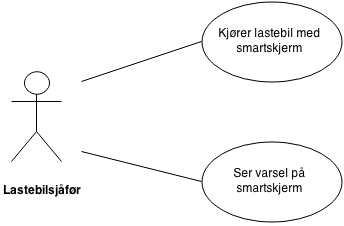
\includegraphics[width=0.50\textwidth]{images/UC1.png}
		\label{fig:UC1}
		\caption{Use case 1: Sjåfør oppager varsel.}
	\end{figure}

\subsection{Analyse av data}
For å analysere dataene som kommer fra en vibrasjonsmåler, så må man ha en ganske avansert og pålitelig software. Dette systemet bruker Fourieranalyse for å skille ut individuelle frekvenser, og et kunnskapsbasert resonneringssystem for å analysere resultatet fra fourieranalysen.


\subsection{Visualisering av data}
%GUI og shit
